\chapter{In-depth User Interface and User Experience Design}
\label{app:depth_ui_ux}

This appendix provides additional documentation for the user interface design process described in Chapter~\ref{user_interface_and_usability}. While the main chapter focuses on the final interface and its usability principles, this appendix presents the earlier design iterations, prototype development, MVP stage, and additional interaction considerations that informed the final design.

\section{Design Methodology and Principles}

Development of the user interface followed an iterative design process, where layout, interaction patterns, and workflow structure were gradually refined throughout the project. Iterative design is widely recommended in user interface development because it allows teams to evaluate design decisions and improve solutions based on testing and practical experience \cite{hartson2012ux}. This approach allowed the design to evolve alongside the technical implementation while maintaining focus on usability and user control.

\methodheading{Iterative and Agile Design Process}

An agile development approach was used, where design and implementation were carried out in parallel. As new features were introduced, the interface was continuously adjusted to support the expanding functionality of the system. The approach aligns with Agile UX practices, where interface decisions are refined through incremental improvements rather than finalized early in development \cite{gothelf2022leanux}. 

Initial wireframes were created in Figma to explore layout and interaction flows before implementation (Appendix~\ref{fig:prototype_loaded}). Wireframing allows designers to quickly test ideas before committing to development \cite{hartson2012ux}. They were used to define the main workflow.

A functional prototype was then implemented to evaluate interaction patterns and identify usability issues in a practical environment. After the prototype stage, the design was refined into a minimum viable product (MVP), where core system functionality was integrated into the interface (Appendix~\ref{fig:mvp_detection}). The interface was also influenced by Safe Media AI's existing system, allowing users familiar with that platform to encounter recognizable layout structures and interaction patterns. This helped support consistency and reduced the learning curve for potential users.

\methodheading{Core Design Principles}

User control over automated processes was a central design principal. Since detection is performed by machine learning models, users must be able to verify, adjust, and override automated results when necessary \cite{hartson2012ux}. The interface supports this through manual highlighting, adjustment of detection settings, removal of incorrect detections, and customization of redaction methods.

Simplicity was also prioritized to reduce cognitive load and allow users to focus on identifying and redacting sensitive information \cite{norman2013design}. The interface therefore emphasizes essential functionality while avoiding unnecessary complexity. This was especially important because users must inspect visual content carefully and should not be distracted by unrelated interface elements.

Visual feedback was prioritized to help users understand system state and detection outcomes \cite{norman2013design}. Detection results are displayed directly on the media using labelled bounding boxes, enabling immediate interpretation of what the system has identified. Progress indicators and visible processing states further help users understand when the system is working.

Consistency across components improves usability and learnability \cite{nielsen2020progressive}. Toolbars, panels, and controls follow predictable patterns, making the interface easier to navigate. In addition, alignment with familiar structures from Safe Media AI's existing system supports recognition for users already accustomed to that platform, while still allowing SafeVision to introduce functionality specific to visual media redaction.

\section{Design Evolution}

The interface evolved through several stages, beginning with simple wireframes and later progressing into a prototype, MVP, and final interface. Each stage was used to explore layout, interaction flow, and the relationship between automated detection and manual user control.

The design was also influenced by Safe Media AI's existing interface. This was done to preserve familiar layout structures and interaction patterns for users already accustomed to that platform, while adapting the workflow to the specific needs of visual media redaction.

The early design stages focused on establishing the main workflow: uploading media, running detection, reviewing results, and applying redaction. Later iterations expanded this into a more complete workspace that supported manual correction, configuration options, visual feedback, and video processing.

\subsection{Initial Design}

Based on the initial requirements and project scope, the first interface design only needed to support a limited set of core functions: uploading an image, detecting sensitive information, and redacting detected content. Because of this limited scope, it was determined early in the design phase that the application did not require multiple pages, pop-up dialogs, or additional navigation views. Instead, the full workflow could be contained within a single interface, allowing users to complete the main redaction process in one place.

The initial interface was centered around a main interaction area for the uploaded image. Before upload, the interface presented a minimal layout with a central upload button, as shown in Figure~\ref{fig:prototype_empty}.

\begin{figure}[H]
\centering
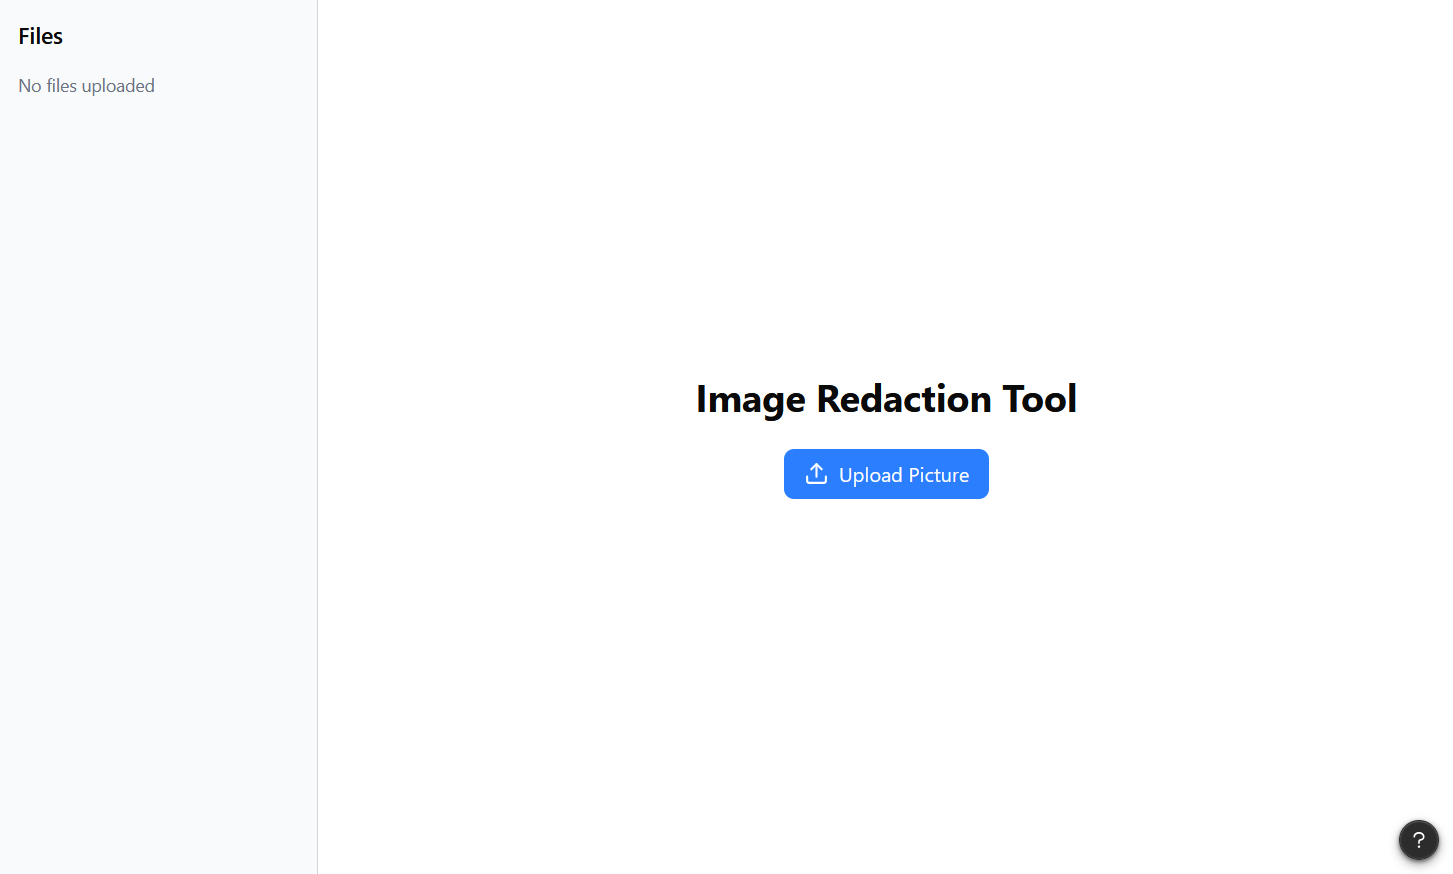
\includegraphics[width=0.8\textwidth]{figures/images/chapter-6/figmasketch3.png}
\caption{Initial interface before an image is uploaded.}
\label{fig:prototype_empty}
\end{figure}

After upload, the layout adapts to include interaction features. The upload button moves to the top, while the central area becomes the image viewer.

A file list is displayed on the left, and control buttons below the viewer allow detection, redaction, and highlighting. This placement maintains a clear connection between the image and available actions, as shown in Figure~\ref{fig:prototype_loaded}.

\begin{figure}[H]
\centering
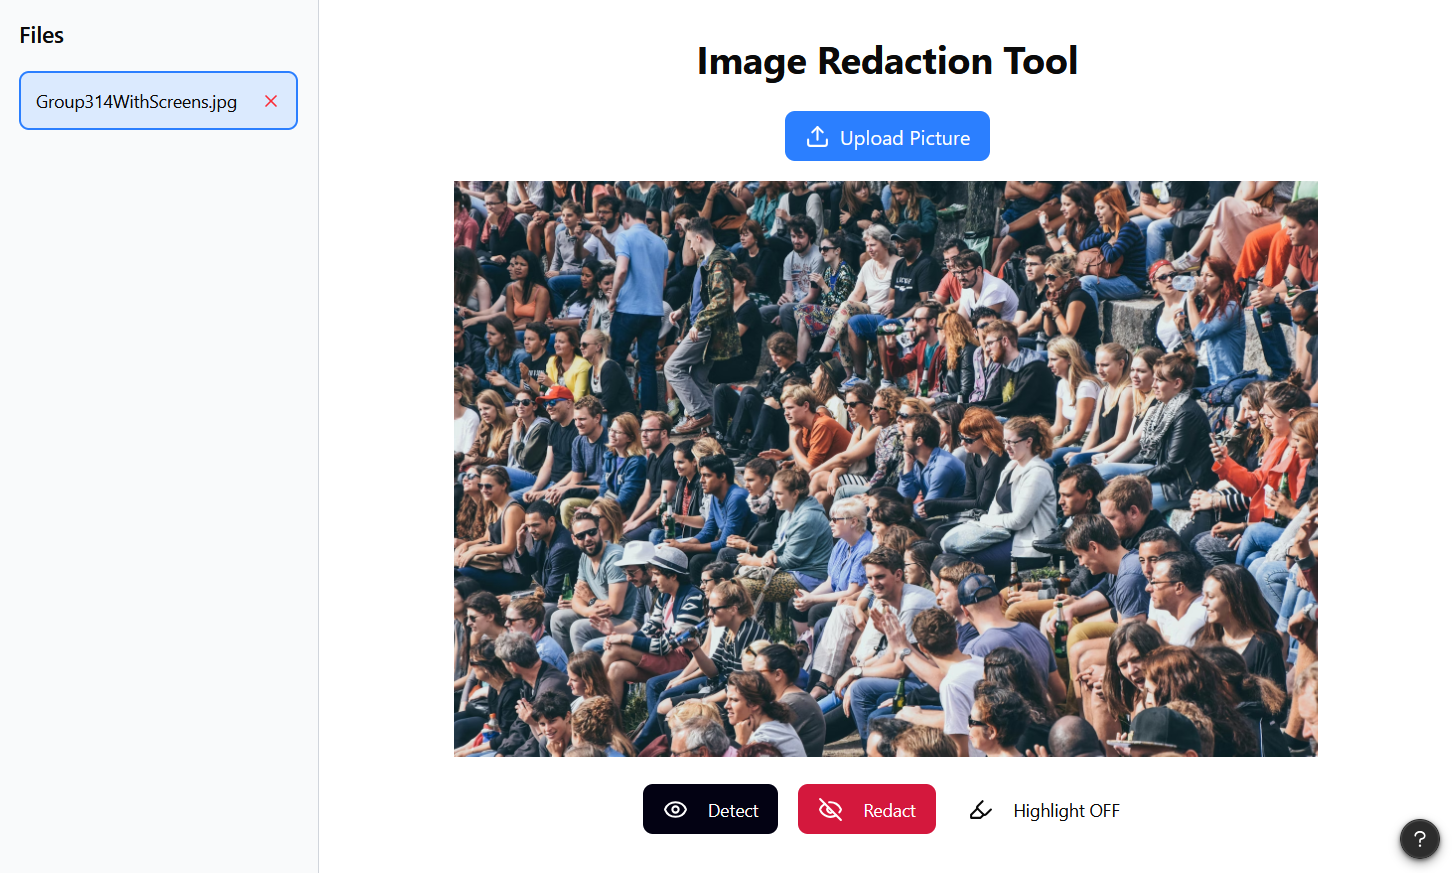
\includegraphics[width=0.8\textwidth]{figures/images/chapter-6/figmasketch4.png}
\caption{Prototype interface after an image has been uploaded.}
\label{fig:prototype_loaded}
\end{figure}

This design provides a clear workflow where users upload an image, run detection, and apply redaction.

\subsection{Prototype}

The prototype was developed in a separate repository to explore layout and interaction patterns without affecting the main system.

Key components such as a sidebar, navigation bar, and central viewer were introduced to structure the interface and organize available tools.

\begin{figure}[H]
\centering
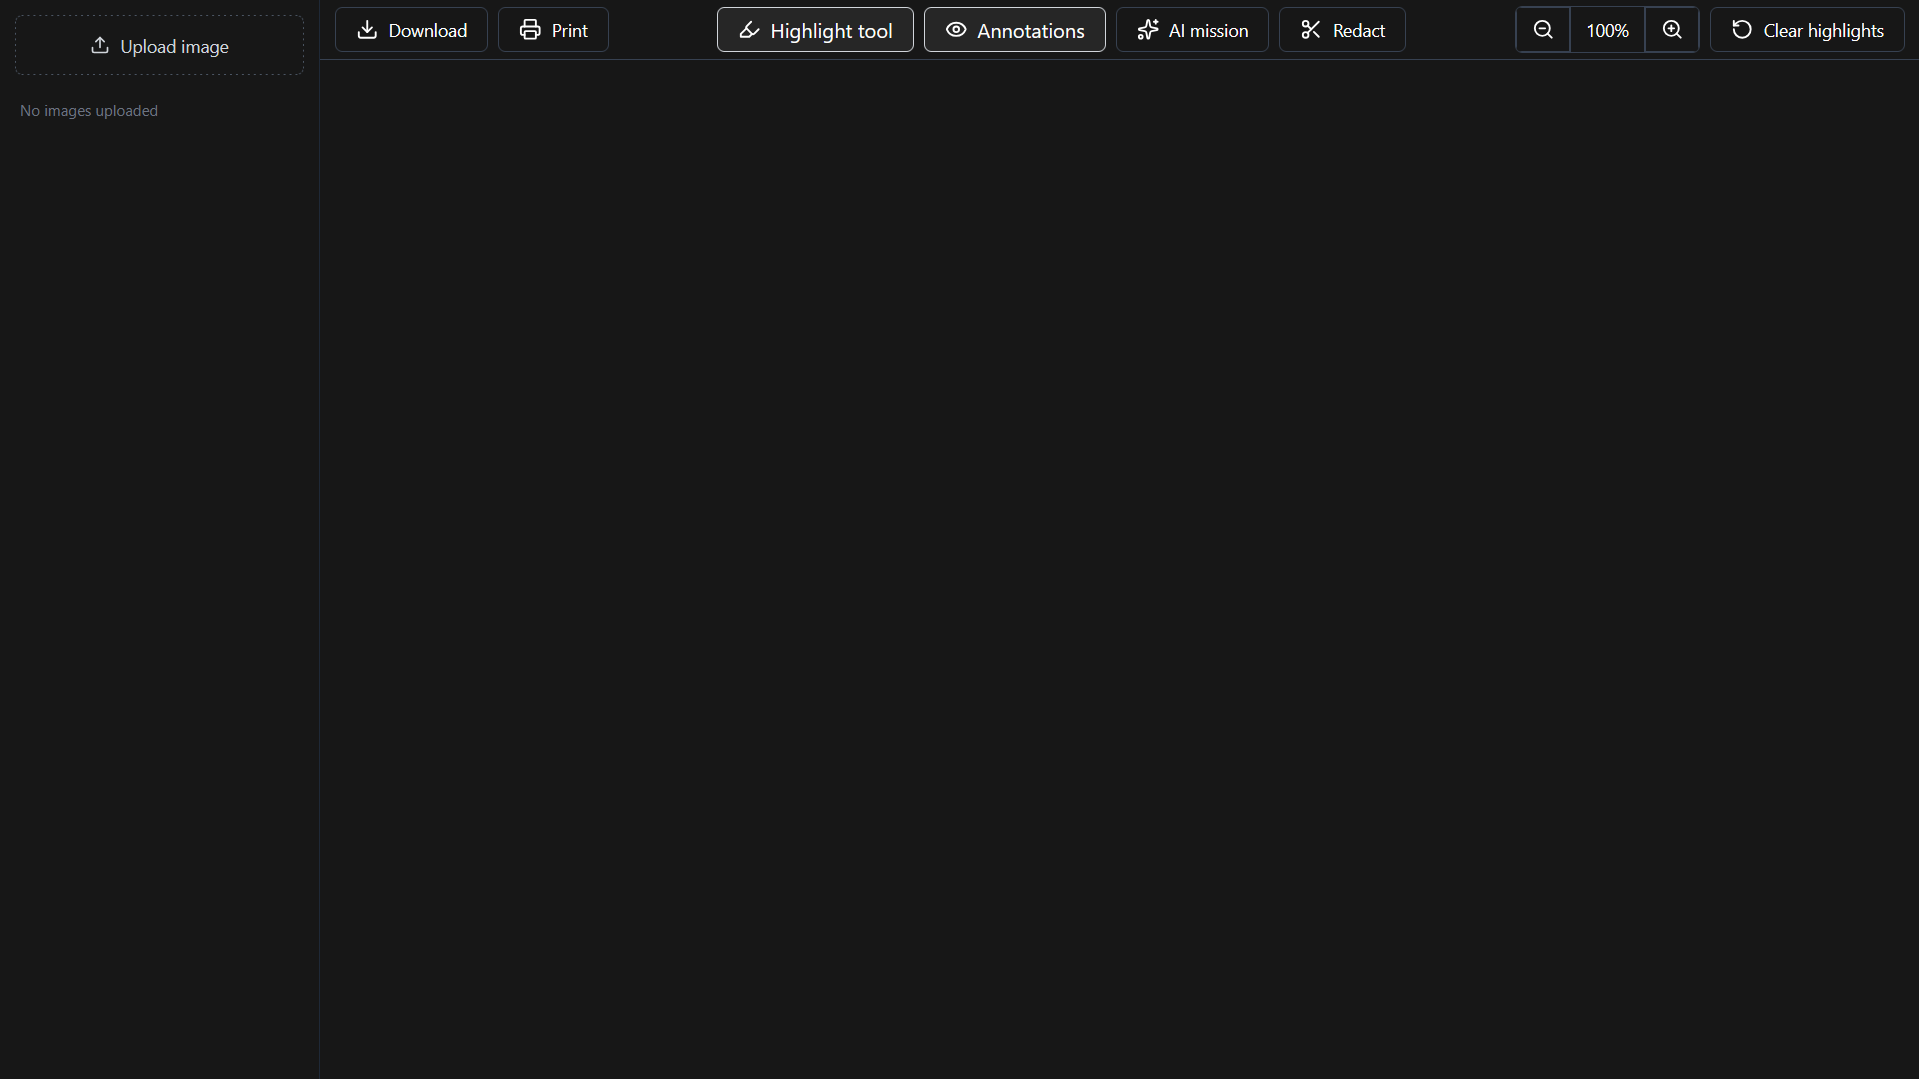
\includegraphics[width=0.8\textwidth]{figures/images/chapter-6/prototype1.png}
\caption{Prototype interface showing the sidebar, navigation bar, and image viewer.}
\label{fig:prototype_overview}
\end{figure}

Some elements were included for layout testing only, such as the \textit{AI Mission} and \textit{Redact} buttons.

The prototype also introduced manual highlighting, allowing users to mark regions directly within the viewer.

\begin{figure}[H]
\centering
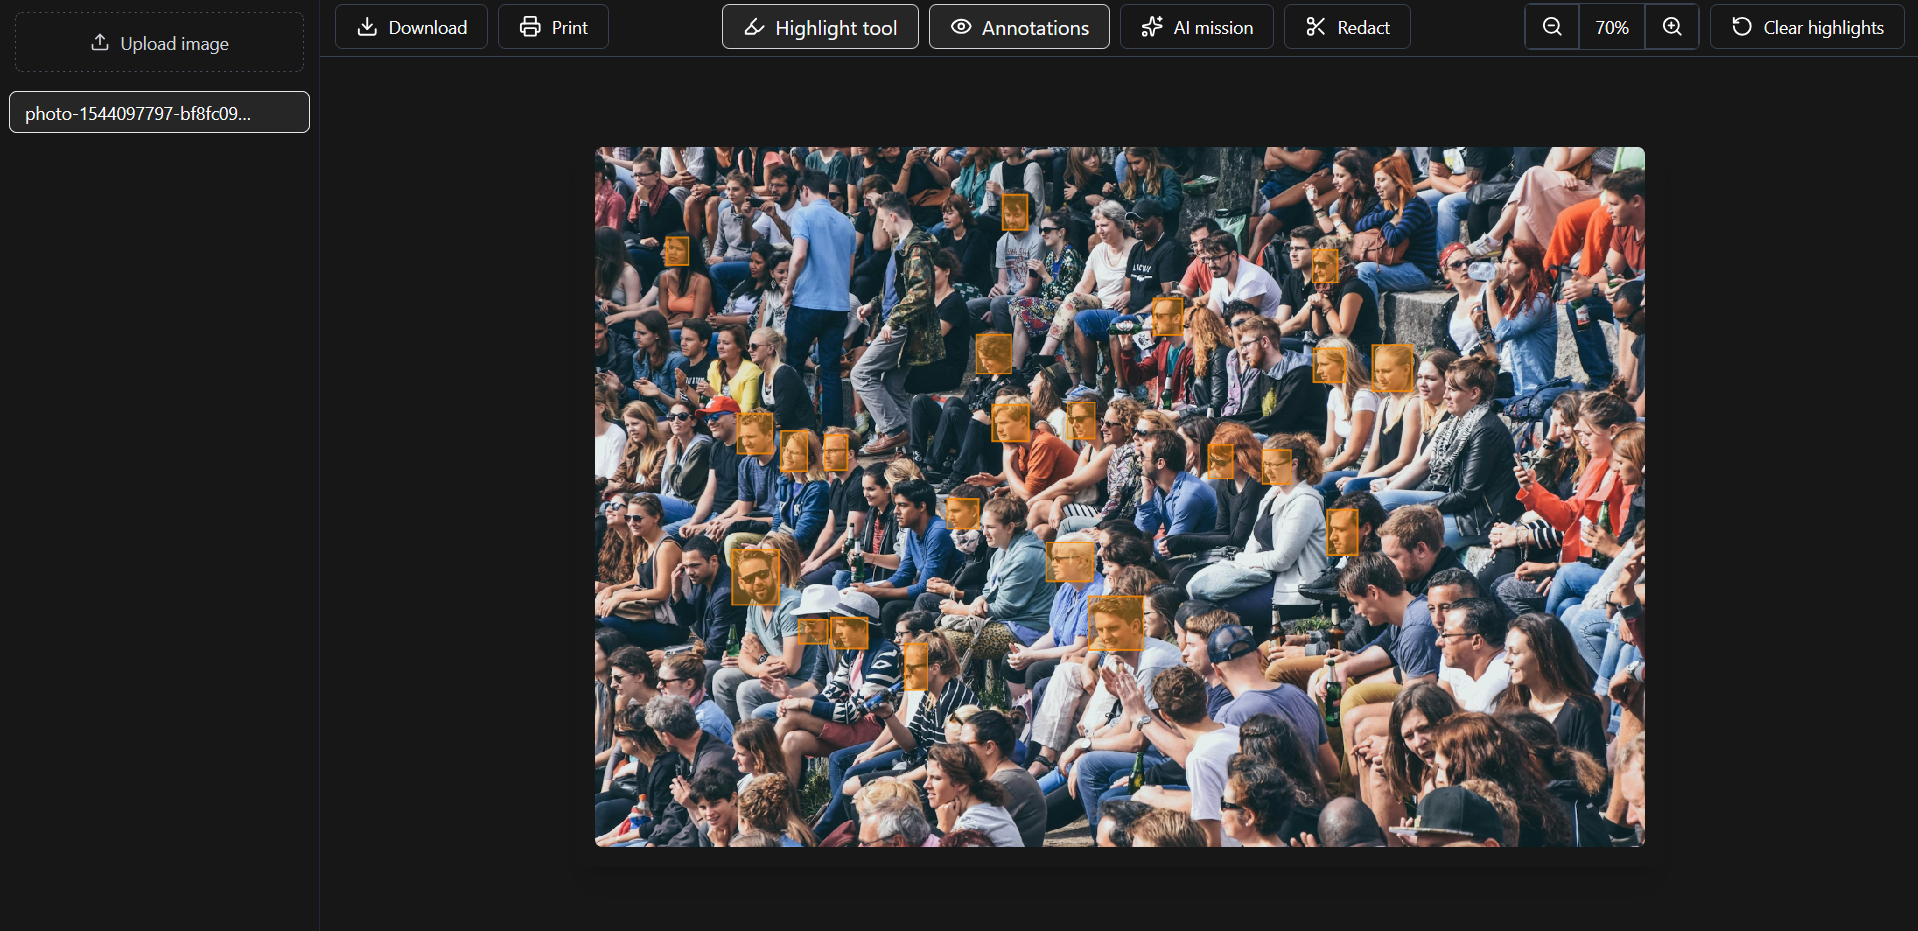
\includegraphics[width=0.7\textwidth]{figures/images/chapter-6/prototype3.png}
\caption{Prototype example showing manually highlighted regions.}
\label{fig:prototype_detection}
\end{figure}

\subsection{MVP Design Iteration}

The MVP introduced functional backend integration while preserving the basic prototype layout, including the sidebar structure and central viewer. Previously inactive interface elements were connected to system functionality, allowing users to run automatic detection and view results as bounding boxes.

At this stage, the interface also explored support for multi-page PDF documents. This allowed users to navigate pages within the same workspace. However, as the project scope evolved, PDF support became less central and the interface was later refocused around image and video redaction.

This iteration was important because it connected the visual interface to actual detection functionality. It also confirmed the need for a human-in-the-loop workflow, where automated detection results are shown visually and can be reviewed before redaction.

\begin{figure}[H]
\centering
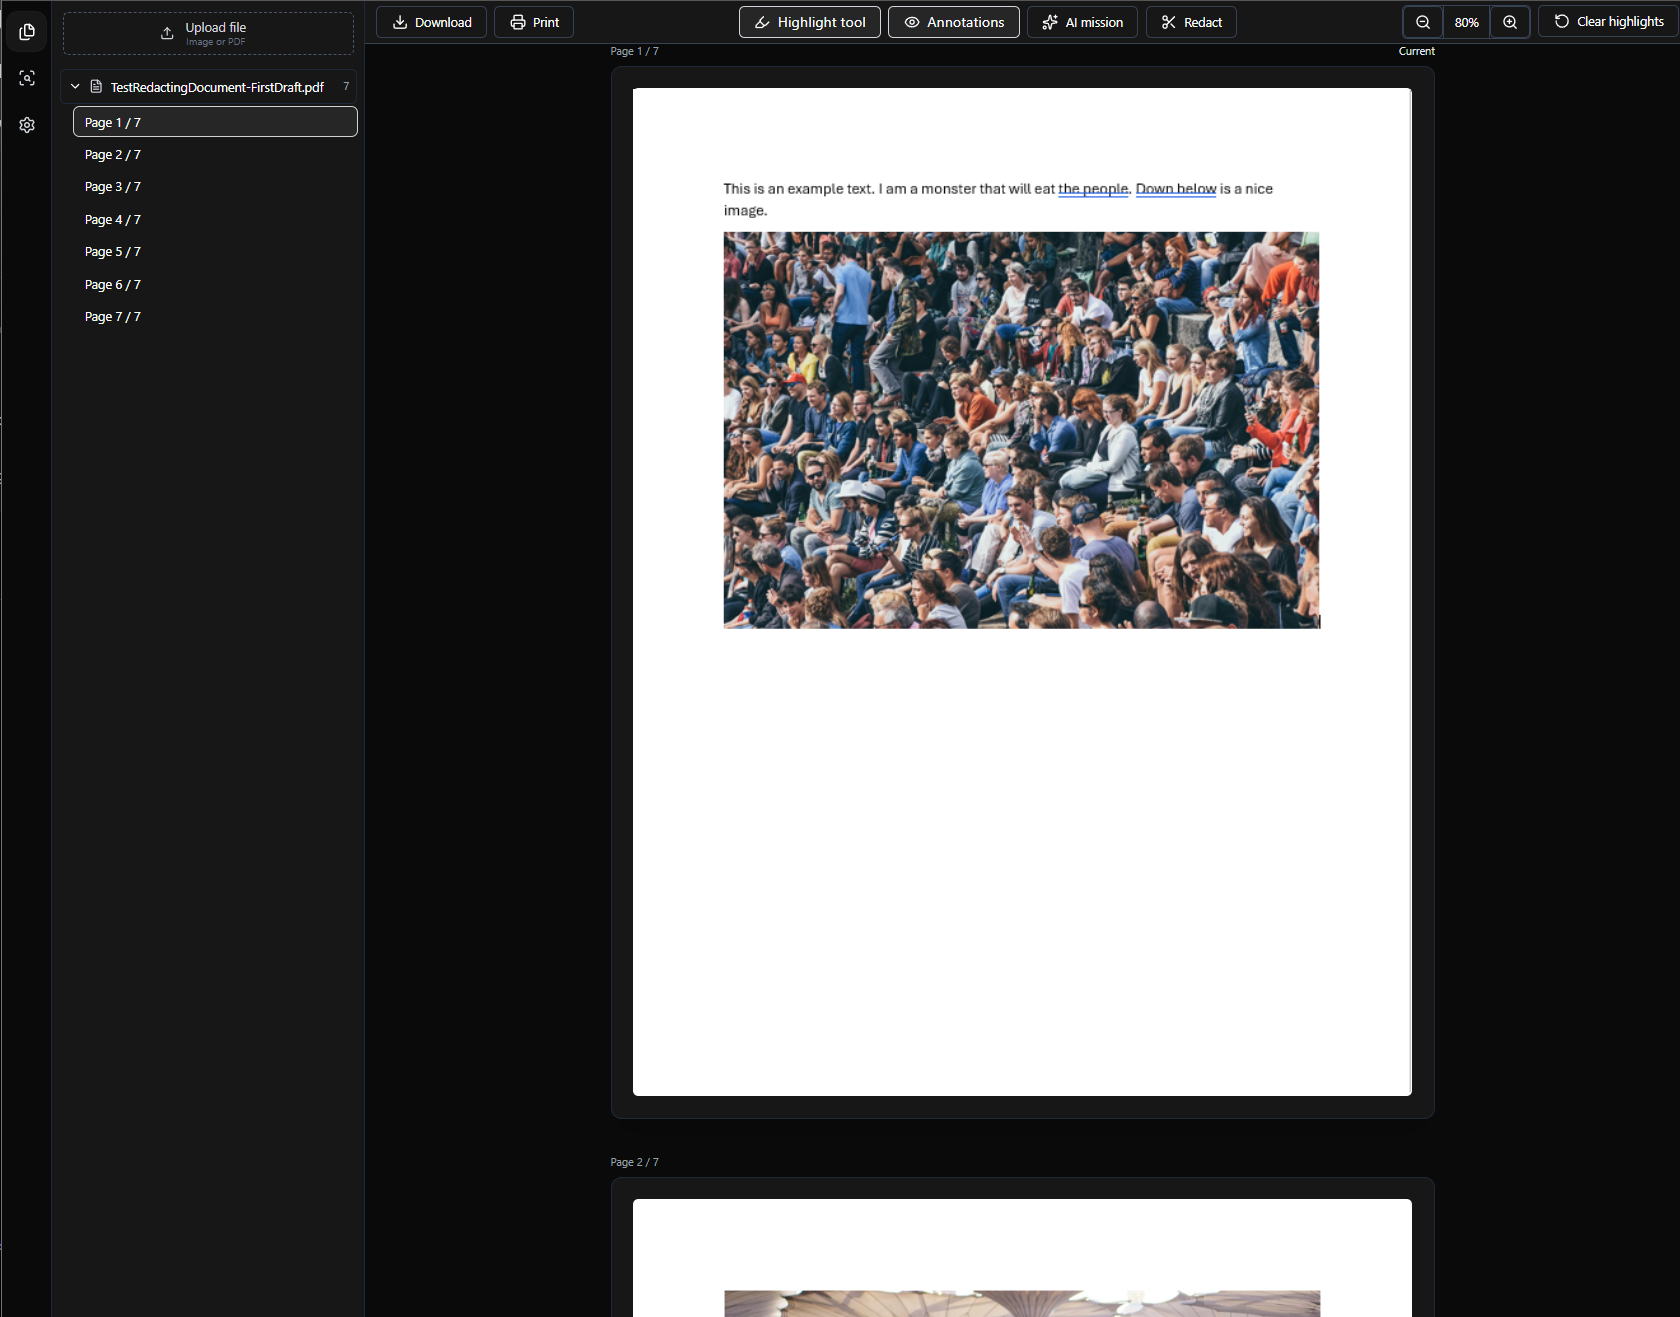
\includegraphics[width=0.8\textwidth]{figures/images/chapter-6/mvp1.png}
\caption{MVP interface showing the document viewer and navigation structure.}
\label{fig:mvp_overview}
\end{figure}

Support for multi-page PDF documents was also introduced, allowing users to navigate pages within the same interface.

\begin{figure}[H]
\centering
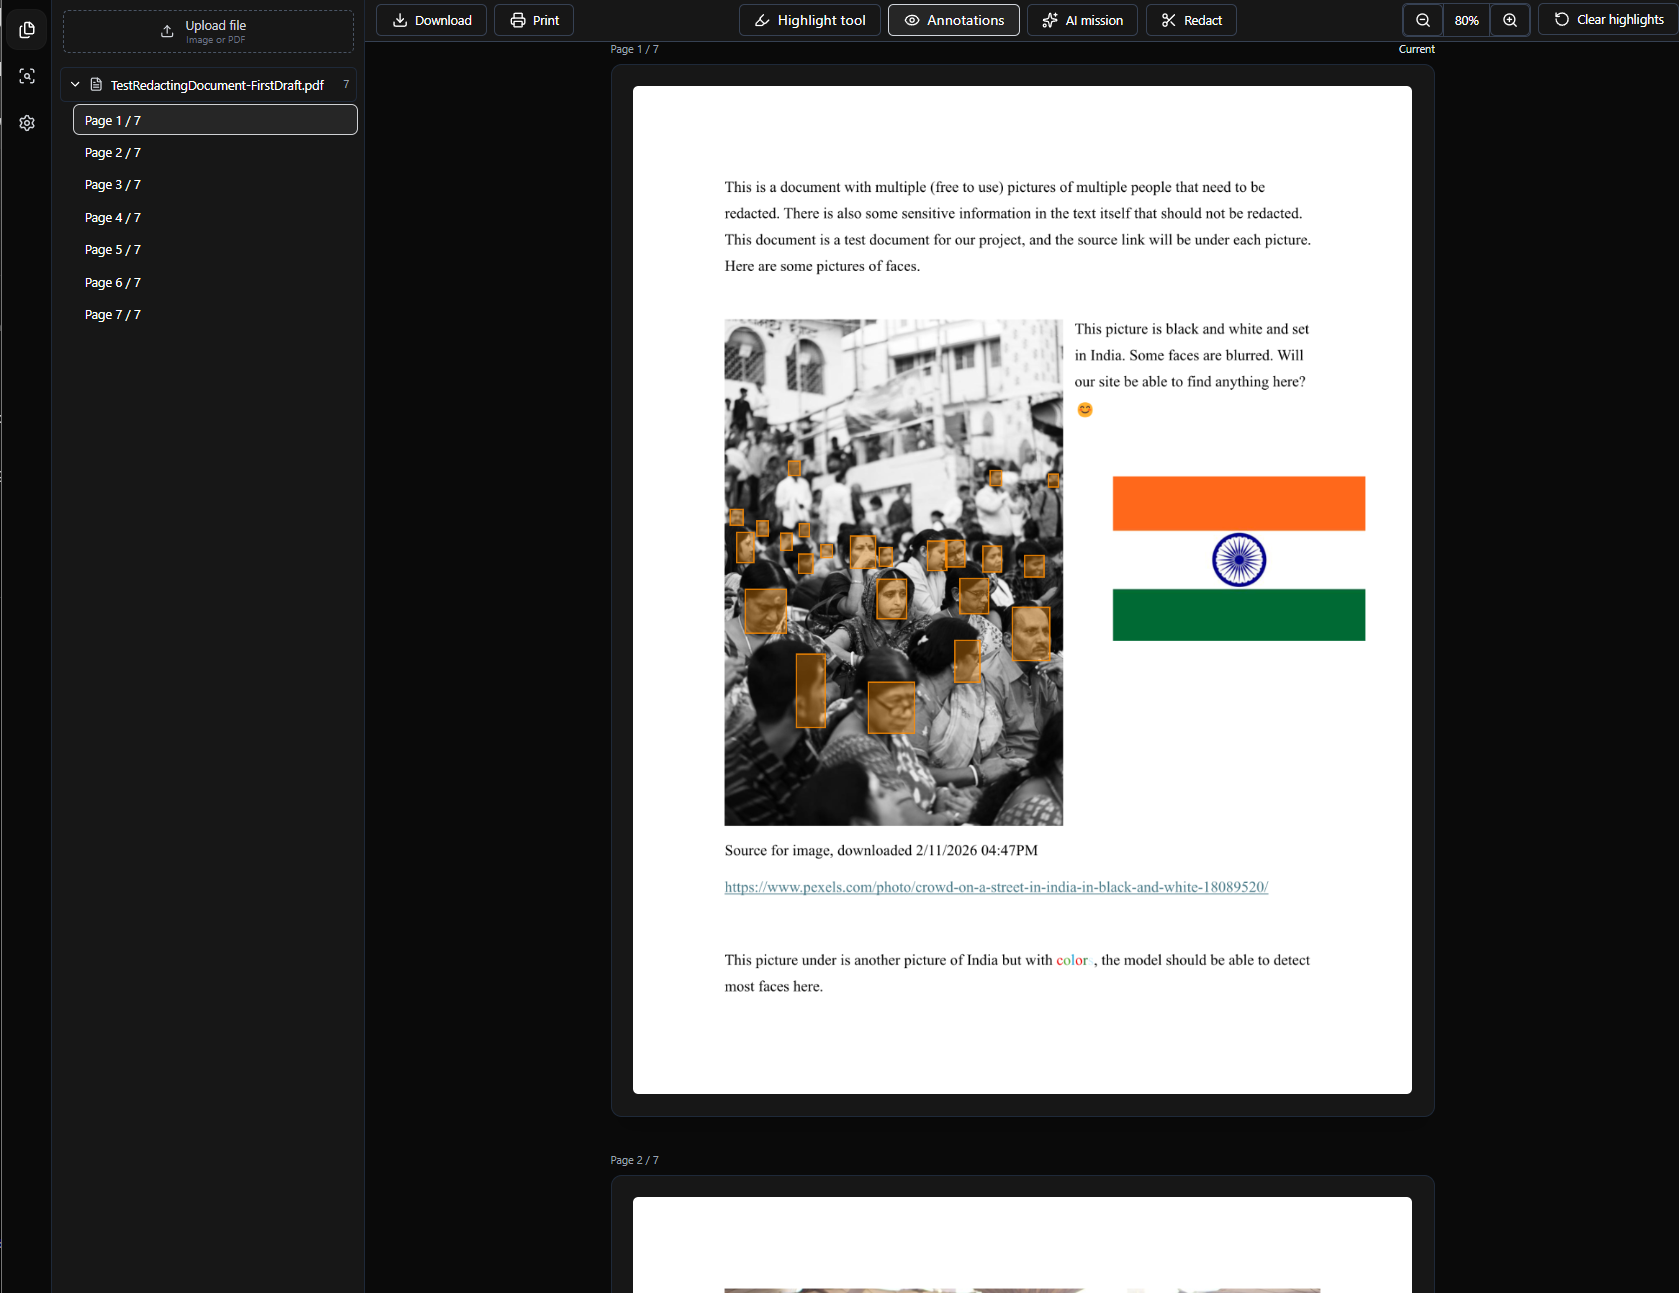
\includegraphics[width=0.8\textwidth]{figures/images/chapter-6/mvp2.png}
\caption{Detection results displayed using bounding boxes.}
\label{fig:mvp_detection}
\end{figure}

This iteration integrates automated detection with manual interaction, enabling users to verify and refine results before applying redaction.

\subsection{Final Design Direction}

The final design refined the interface into a focused workspace for image and video redaction. Compared with earlier iterations, the layout was simplified to reduce visual complexity and improve usability. The final interface retained the central viewer and side-panel structure, but reorganized controls so that upload, identification, review, correction, and redaction could be completed in a more natural sequence.

As the project evolved, support for PDF workflows was reduced, while video processing capabilities were introduced. This required the interface to support temporal media through playback controls, frame-based inspection, and detection overlays on video frames. A Terms of Service component was also implemented to address privacy and data protection requirements before users interact with the system.

The final interface and its components are described in the main text in Section~\ref{user_interface_and_usability}. This appendix therefore focuses on documenting the design progression that led to the final solution.

\section{Usability and Interaction Design}

This section focuses specifically on the interaction between the user and the machine learning-based detection and redaction functionality. While the interface includes several general usability features, the primary objective of the system is to support a human-in-the-loop workflow. Therefore, the usability discussion is centered on how users interact with detection results, verify automated outputs, and apply redaction.

\subsection{Interaction with Detection Results}

The core interaction in the system occurs within the document viewer, where detection results are presented directly on the image using bounding boxes. This allows users to immediately interpret the output of the detection models and understand which regions have been identified as potentially sensitive.

Since machine learning models are not perfectly accurate, it is essential that users can validate these results. The interface therefore allows users to manually adjust bounding boxes, remove incorrect detections, and add new regions if necessary. This ensures that the final outcome is not solely dependent on automated predictions, but can be refined through user input.

By combining automatic detection with manual correction, the system supports a more reliable and controllable redaction process.

\subsection{Detection Configuration and Control}

Users are able to control the detection process by selecting which categories of sensitive information to detect. This allows the system to be adapted to different use cases, where only specific types of content may be relevant.

Providing this level of control reduces unnecessary visual clutter and improves usability by ensuring that users only see relevant detection results. It also allows users to tailor the system behavior to the specific context of the document or image being processed.

\subsection{Redaction Interaction}

Once detection results have been reviewed, users can apply redaction directly within the interface. Multiple redaction methods are available, including black box redaction, blur, and pixelation.

Allowing users to select and adjust redaction methods provides flexibility in how sensitive information is concealed. For example, blur and pixelation may preserve some visual context, while solid redaction completely removes visibility. This enables users to choose the most appropriate method depending on the sensitivity of the content.

The integration of redaction controls within the same workspace as detection results ensures a seamless workflow, where users can move directly from analysis to action without changing context.

\subsection{Visual Feedback for Verification}

Clear visual feedback is essential when interacting with automated detection systems. In the interface, detection results are displayed as overlays on the document, allowing users to quickly assess model outputs.

This immediate feedback supports rapid verification, as users can visually confirm whether detected regions correspond to actual sensitive content. Any inaccuracies can then be corrected before redaction is applied.

By providing continuous visual feedback throughout the workflow, the interface helps users maintain awareness of system behavior and increases confidence in the final result.

\subsection{Accessibility Considerations}

Accessibility considerations were integrated into the interaction design to support effective use of detection and redaction tasks over extended periods. Since the system requires detailed visual inspection, emphasis was placed on reducing visual strain and enabling flexible interaction.

Visual accessibility is supported through dark and light modes, allowing adaptation to different lighting conditions. Users can also customize highlight colors for detection results and manual annotations, improving readability and distinction between detection categories. Zoom functionality further enables detailed inspection of small regions without losing context.

Interaction accessibility is addressed through flexible input methods. Keyboard shortcuts support efficient interaction during repetitive tasks, while undo and redo functionality allow users to safely adjust detection results and redaction without risk of permanent errors.

Together, these features improve usability, flexibility, and efficiency in the human-in-the-loop redaction workflow.

\methodheading{Terms of Services}
\label{app:terms_of_service}

A Terms of Service dialog was included in the final interface to clarify user responsibility, acceptable use, data handling, and the limitations of automated redaction. The text below summarizes the terms shown to users before processing content in \gls{SafeVision}.

\begin{enumerate}
    \item \textbf{Operator and contact:} The service is operated by An Hoang Chu, Karwan Shekhe, and Henrik Weflen Gjermundsen. Contact: henrik.w.gjermundsen@gmail.com.

    \item \textbf{What the service does:} The service provides automated detection and redaction functionality to help redact images. Automated detection may be inaccurate or incomplete.

    \item \textbf{User responsibilities and acceptable use:} Users confirm that they have the necessary rights and a valid legal basis to upload and process any personal data contained in the content they submit. Users must not upload unlawful content or content that infringes the rights or privacy of others. Users must not upload content involving children or other vulnerable individuals unless they are legally authorised to do so. Users are responsible for reviewing the output before sharing, publishing, or otherwise using it, because redaction may be imperfect. Access may be blocked or restricted if there is reasonable belief that the service is being misused or used unlawfully.

    \item \textbf{How images are processed, stored, and deleted:} When an image or document is uploaded, it is transmitted to the backend servers and processed by the system to detect sensitive content and apply redaction. The servers are hosted on infrastructure provided by Google Cloud. Uploaded images and redacted outputs are not stored permanently. Uploads are used only to generate the result and are deleted after the result is returned, although transient technical handling may occur during processing and delivery. Uploaded content is not used to train or improve the model.

    \item \textbf{Browser-stored backtracking and cached box data:} To support editing features, the web application stores derived detection data in the user's browser on the user's device. This may include bounding-box coordinates, image dimensions, and related redaction or editing state. The service uses an in-memory undo and redo history during the session, as well as local browser storage or cache to restore detected boxes and editing state when the user revisits the site. This browser-stored data does not include the original uploaded image. Users can remove this data at any time by clearing the site's data in their browser.

    \item \textbf{Logging:} The service does not intentionally log or retain uploaded image content. Some infrastructure-level operational data may be processed transiently to deliver the service.

    \item \textbf{Rights and complaints:} For questions or data protection requests, users can contact henrik.w.gjermundsen@gmail.com. Users may also lodge a complaint with their supervisory authority, Datatilsynet.

    \item \textbf{Disclaimer:} The service is provided ``as is'' and ``as available.'' The system does not guarantee that all sensitive content will be detected or redacted. Users are responsible for verifying outputs before sharing or publishing. Nothing in these terms limits liability where such limitation is not permitted by law.
\end{enumerate}


